% Options for packages loaded elsewhere
\PassOptionsToPackage{unicode}{hyperref}
\PassOptionsToPackage{hyphens}{url}
%
\documentclass[
]{article}
\title{R journal examples}
\author{}
\date{\vspace{-2.5em}}

\usepackage{amsmath,amssymb}
\usepackage{lmodern}
\usepackage{iftex}
\ifPDFTeX
  \usepackage[T1]{fontenc}
  \usepackage[utf8]{inputenc}
  \usepackage{textcomp} % provide euro and other symbols
\else % if luatex or xetex
  \usepackage{unicode-math}
  \defaultfontfeatures{Scale=MatchLowercase}
  \defaultfontfeatures[\rmfamily]{Ligatures=TeX,Scale=1}
\fi
% Use upquote if available, for straight quotes in verbatim environments
\IfFileExists{upquote.sty}{\usepackage{upquote}}{}
\IfFileExists{microtype.sty}{% use microtype if available
  \usepackage[]{microtype}
  \UseMicrotypeSet[protrusion]{basicmath} % disable protrusion for tt fonts
}{}
\makeatletter
\@ifundefined{KOMAClassName}{% if non-KOMA class
  \IfFileExists{parskip.sty}{%
    \usepackage{parskip}
  }{% else
    \setlength{\parindent}{0pt}
    \setlength{\parskip}{6pt plus 2pt minus 1pt}}
}{% if KOMA class
  \KOMAoptions{parskip=half}}
\makeatother
\usepackage{xcolor}
\IfFileExists{xurl.sty}{\usepackage{xurl}}{} % add URL line breaks if available
\IfFileExists{bookmark.sty}{\usepackage{bookmark}}{\usepackage{hyperref}}
\hypersetup{
  pdftitle={R journal examples},
  hidelinks,
  pdfcreator={LaTeX via pandoc}}
\urlstyle{same} % disable monospaced font for URLs
\usepackage[margin=1in]{geometry}
\usepackage{color}
\usepackage{fancyvrb}
\newcommand{\VerbBar}{|}
\newcommand{\VERB}{\Verb[commandchars=\\\{\}]}
\DefineVerbatimEnvironment{Highlighting}{Verbatim}{commandchars=\\\{\}}
% Add ',fontsize=\small' for more characters per line
\usepackage{framed}
\definecolor{shadecolor}{RGB}{248,248,248}
\newenvironment{Shaded}{\begin{snugshade}}{\end{snugshade}}
\newcommand{\AlertTok}[1]{\textcolor[rgb]{0.94,0.16,0.16}{#1}}
\newcommand{\AnnotationTok}[1]{\textcolor[rgb]{0.56,0.35,0.01}{\textbf{\textit{#1}}}}
\newcommand{\AttributeTok}[1]{\textcolor[rgb]{0.77,0.63,0.00}{#1}}
\newcommand{\BaseNTok}[1]{\textcolor[rgb]{0.00,0.00,0.81}{#1}}
\newcommand{\BuiltInTok}[1]{#1}
\newcommand{\CharTok}[1]{\textcolor[rgb]{0.31,0.60,0.02}{#1}}
\newcommand{\CommentTok}[1]{\textcolor[rgb]{0.56,0.35,0.01}{\textit{#1}}}
\newcommand{\CommentVarTok}[1]{\textcolor[rgb]{0.56,0.35,0.01}{\textbf{\textit{#1}}}}
\newcommand{\ConstantTok}[1]{\textcolor[rgb]{0.00,0.00,0.00}{#1}}
\newcommand{\ControlFlowTok}[1]{\textcolor[rgb]{0.13,0.29,0.53}{\textbf{#1}}}
\newcommand{\DataTypeTok}[1]{\textcolor[rgb]{0.13,0.29,0.53}{#1}}
\newcommand{\DecValTok}[1]{\textcolor[rgb]{0.00,0.00,0.81}{#1}}
\newcommand{\DocumentationTok}[1]{\textcolor[rgb]{0.56,0.35,0.01}{\textbf{\textit{#1}}}}
\newcommand{\ErrorTok}[1]{\textcolor[rgb]{0.64,0.00,0.00}{\textbf{#1}}}
\newcommand{\ExtensionTok}[1]{#1}
\newcommand{\FloatTok}[1]{\textcolor[rgb]{0.00,0.00,0.81}{#1}}
\newcommand{\FunctionTok}[1]{\textcolor[rgb]{0.00,0.00,0.00}{#1}}
\newcommand{\ImportTok}[1]{#1}
\newcommand{\InformationTok}[1]{\textcolor[rgb]{0.56,0.35,0.01}{\textbf{\textit{#1}}}}
\newcommand{\KeywordTok}[1]{\textcolor[rgb]{0.13,0.29,0.53}{\textbf{#1}}}
\newcommand{\NormalTok}[1]{#1}
\newcommand{\OperatorTok}[1]{\textcolor[rgb]{0.81,0.36,0.00}{\textbf{#1}}}
\newcommand{\OtherTok}[1]{\textcolor[rgb]{0.56,0.35,0.01}{#1}}
\newcommand{\PreprocessorTok}[1]{\textcolor[rgb]{0.56,0.35,0.01}{\textit{#1}}}
\newcommand{\RegionMarkerTok}[1]{#1}
\newcommand{\SpecialCharTok}[1]{\textcolor[rgb]{0.00,0.00,0.00}{#1}}
\newcommand{\SpecialStringTok}[1]{\textcolor[rgb]{0.31,0.60,0.02}{#1}}
\newcommand{\StringTok}[1]{\textcolor[rgb]{0.31,0.60,0.02}{#1}}
\newcommand{\VariableTok}[1]{\textcolor[rgb]{0.00,0.00,0.00}{#1}}
\newcommand{\VerbatimStringTok}[1]{\textcolor[rgb]{0.31,0.60,0.02}{#1}}
\newcommand{\WarningTok}[1]{\textcolor[rgb]{0.56,0.35,0.01}{\textbf{\textit{#1}}}}
\usepackage{graphicx}
\makeatletter
\def\maxwidth{\ifdim\Gin@nat@width>\linewidth\linewidth\else\Gin@nat@width\fi}
\def\maxheight{\ifdim\Gin@nat@height>\textheight\textheight\else\Gin@nat@height\fi}
\makeatother
% Scale images if necessary, so that they will not overflow the page
% margins by default, and it is still possible to overwrite the defaults
% using explicit options in \includegraphics[width, height, ...]{}
\setkeys{Gin}{width=\maxwidth,height=\maxheight,keepaspectratio}
% Set default figure placement to htbp
\makeatletter
\def\fps@figure{htbp}
\makeatother
\setlength{\emergencystretch}{3em} % prevent overfull lines
\providecommand{\tightlist}{%
  \setlength{\itemsep}{0pt}\setlength{\parskip}{0pt}}
\setcounter{secnumdepth}{-\maxdimen} % remove section numbering
\ifLuaTeX
  \usepackage{selnolig}  % disable illegal ligatures
\fi

\begin{document}
\maketitle

\hypertarget{smoking-cessation-example}{%
\subsection{Smoking cessation example}\label{smoking-cessation-example}}

\begin{Shaded}
\begin{Highlighting}[]
\FunctionTok{data}\NormalTok{(Smoking)}

\NormalTok{treats }\OtherTok{\textless{}{-}} \FunctionTok{c}\NormalTok{(}\StringTok{"No intervention"}\NormalTok{, }\StringTok{"Self{-}help"}\NormalTok{, }\StringTok{"Individual counselling"}\NormalTok{, }\StringTok{"Group counselling"}\NormalTok{)}
\NormalTok{bcea\_smoke }\OtherTok{\textless{}{-}} \FunctionTok{bcea}\NormalTok{(e, c, }\AttributeTok{ref =} \DecValTok{4}\NormalTok{, }\AttributeTok{interventions =}\NormalTok{ treats, }\AttributeTok{Kmax =} \DecValTok{500}\NormalTok{)}
\end{Highlighting}
\end{Shaded}

grid of plots

\begin{Shaded}
\begin{Highlighting}[]
\FunctionTok{library}\NormalTok{(ggplot2)}

\FunctionTok{plot}\NormalTok{(bcea\_smoke)}
\end{Highlighting}
\end{Shaded}

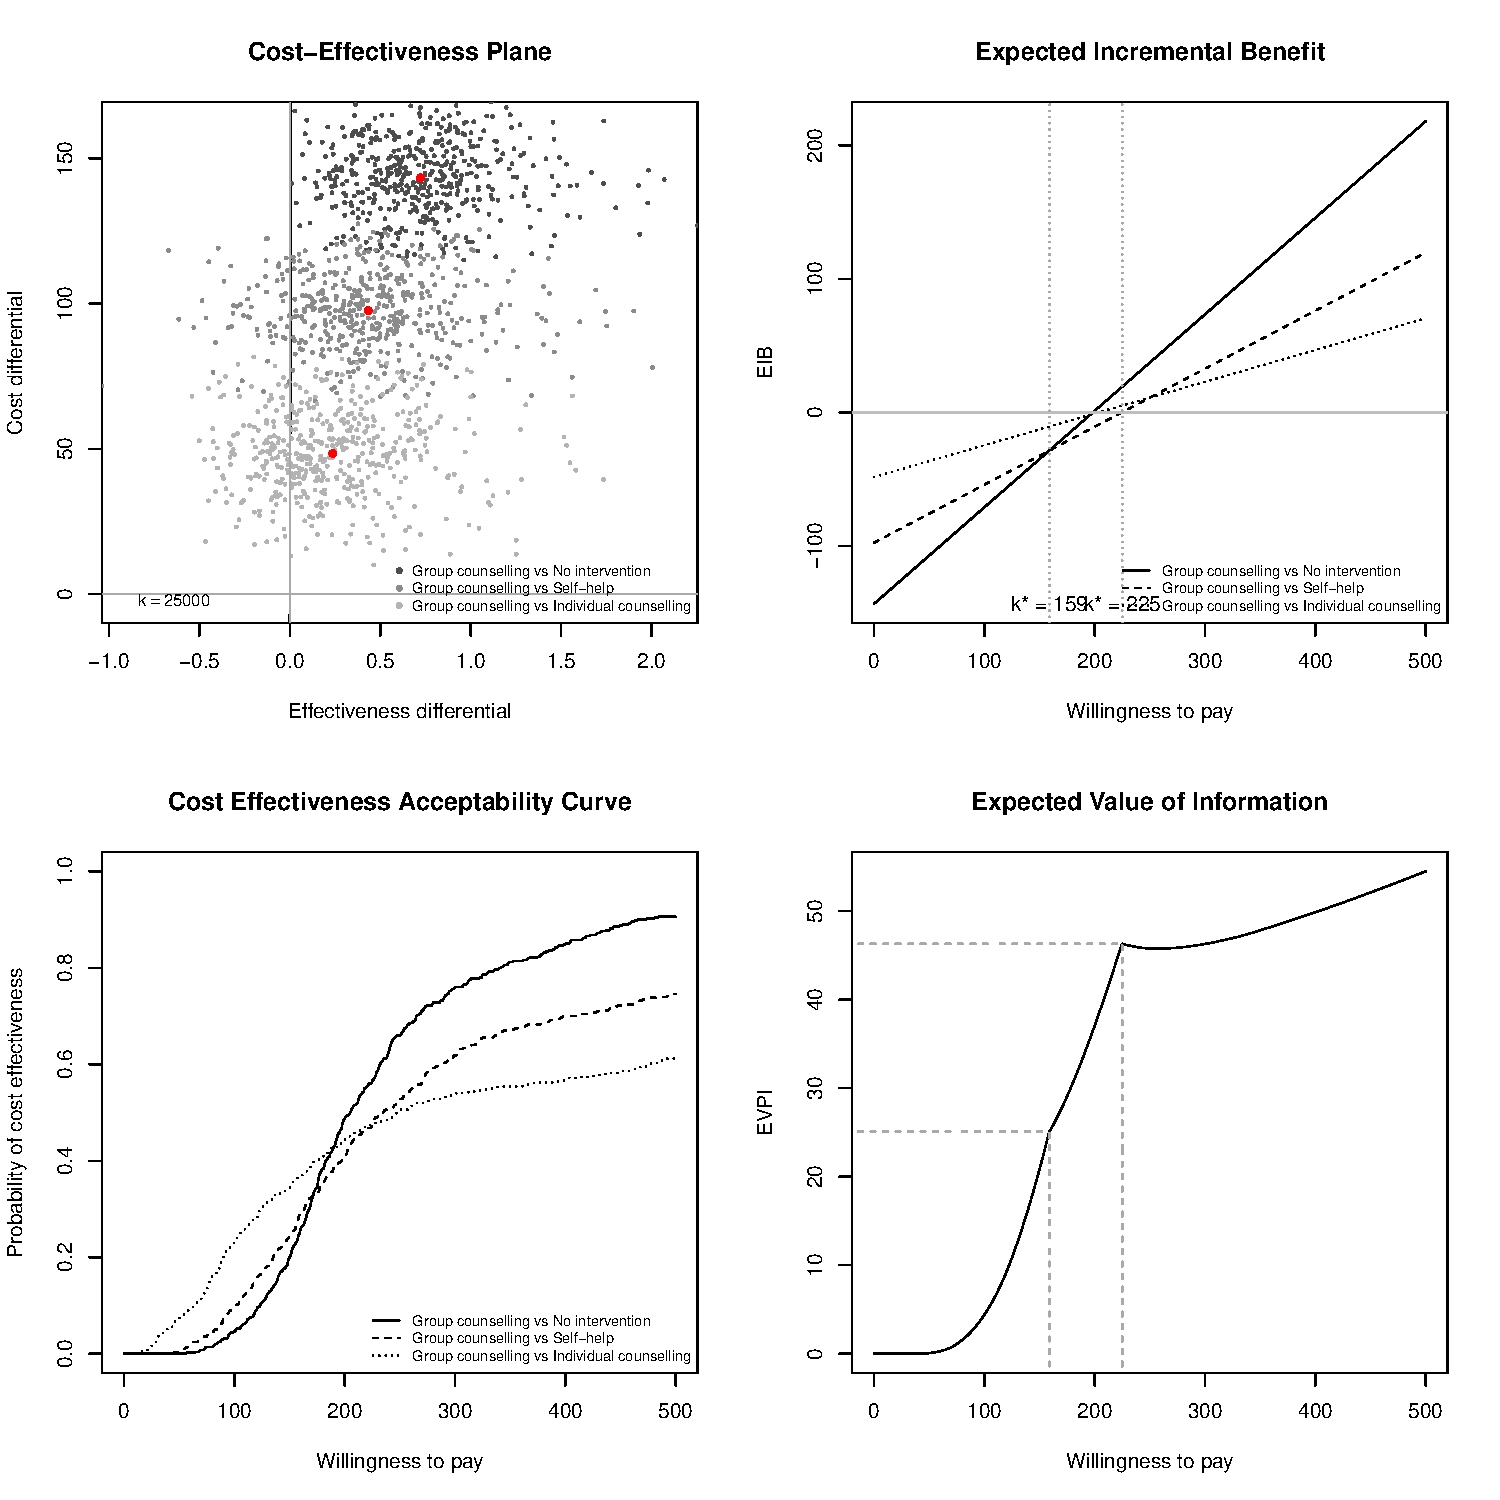
\includegraphics{C:/Users/n8tha/Documents/R/BCEA/vignettes/R_journal_examples_files/figure-latex/unnamed-chunk-4-1.pdf}

\begin{Shaded}
\begin{Highlighting}[]

\FunctionTok{plot}\NormalTok{(bcea\_smoke, }\AttributeTok{graph =} \StringTok{"ggplot2"}\NormalTok{, }\AttributeTok{wtp =} \DecValTok{250}\NormalTok{, }\AttributeTok{pos =} \ConstantTok{TRUE}\NormalTok{, }\AttributeTok{size =} \FunctionTok{rel}\NormalTok{(}\DecValTok{2}\NormalTok{), }\AttributeTok{ICER.size =} \DecValTok{2}\NormalTok{)}
\end{Highlighting}
\end{Shaded}

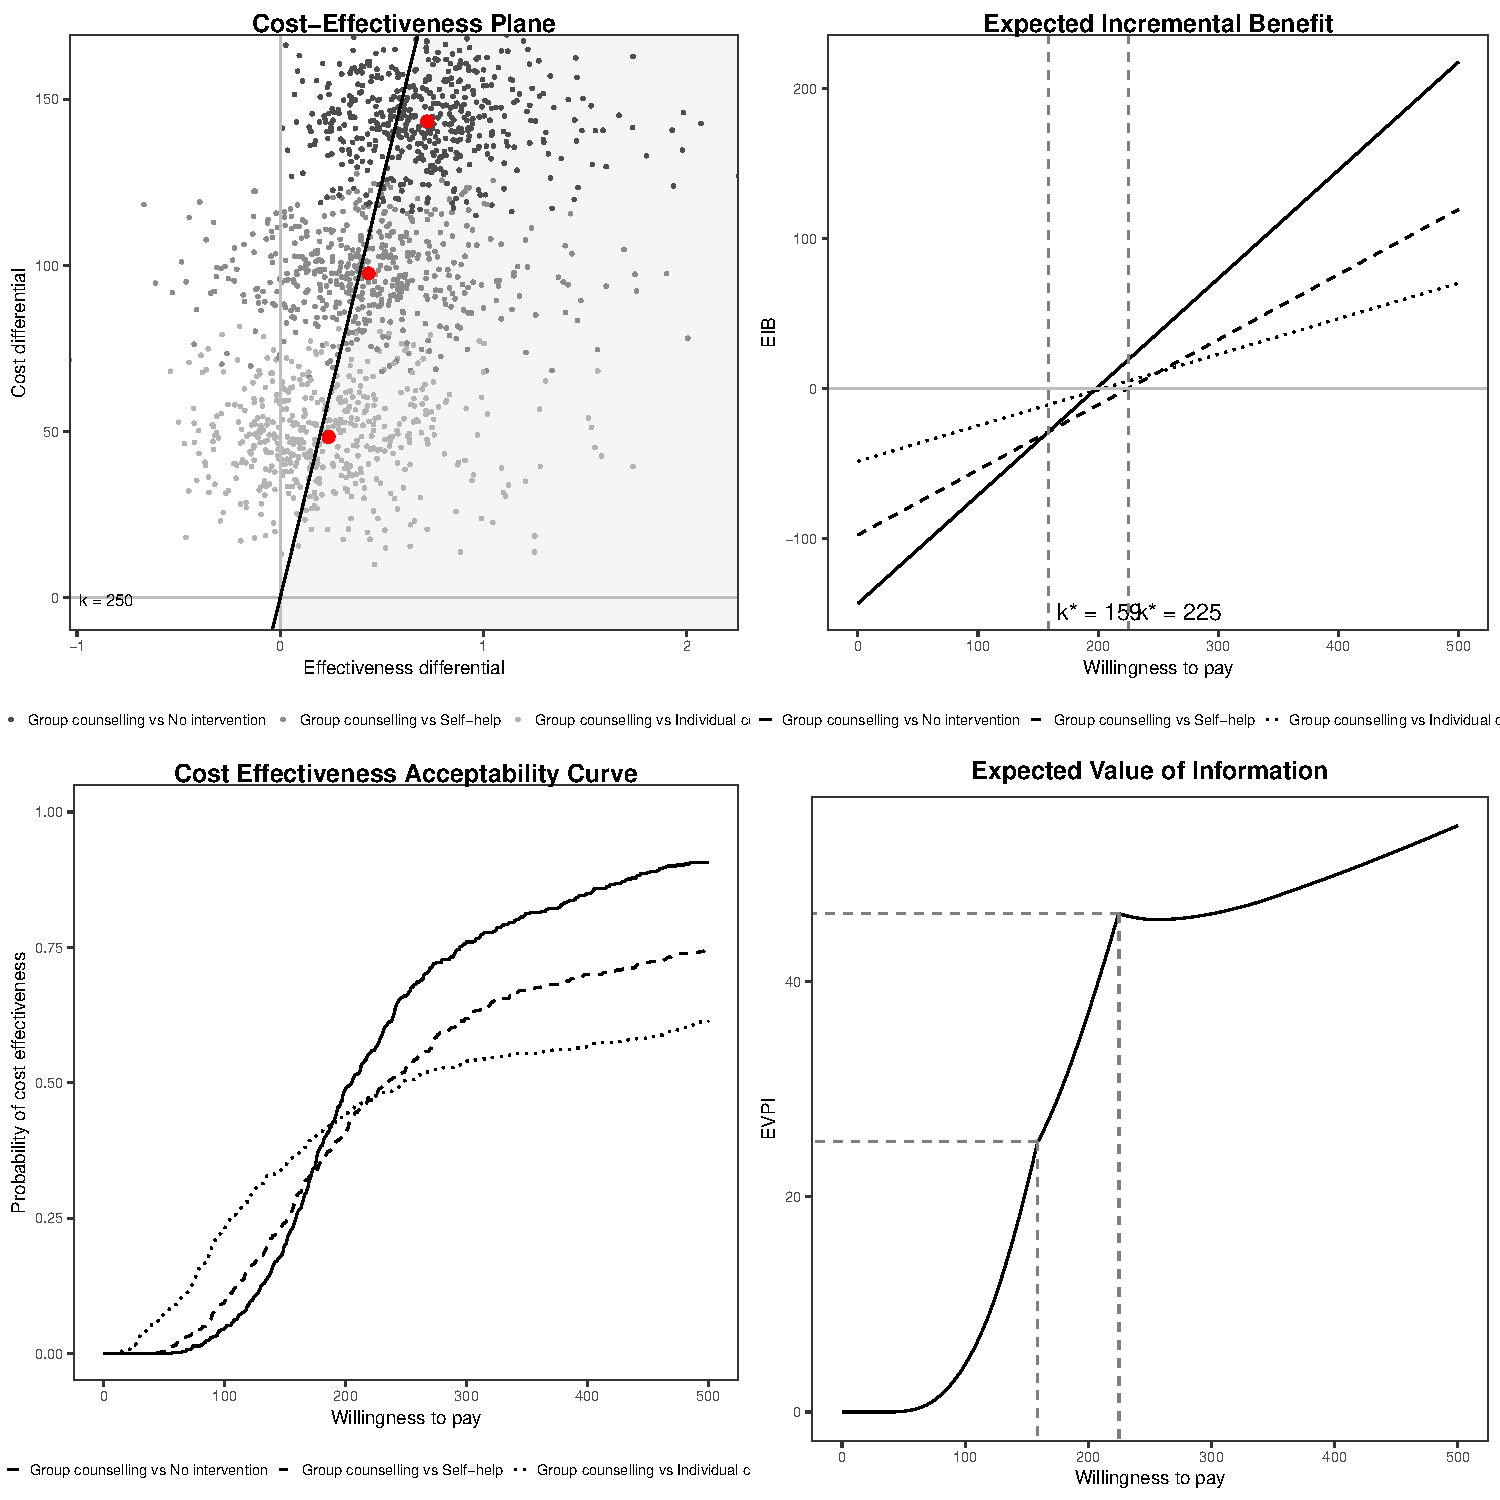
\includegraphics{C:/Users/n8tha/Documents/R/BCEA/vignettes/R_journal_examples_files/figure-latex/unnamed-chunk-4-2.pdf}

individual plots cost-effectiveness plane

\begin{Shaded}
\begin{Highlighting}[]
\FunctionTok{ceplane.plot}\NormalTok{(bcea\_smoke, }\AttributeTok{comparison =} \DecValTok{2}\NormalTok{, }\AttributeTok{wtp =} \DecValTok{250}\NormalTok{)}
\end{Highlighting}
\end{Shaded}

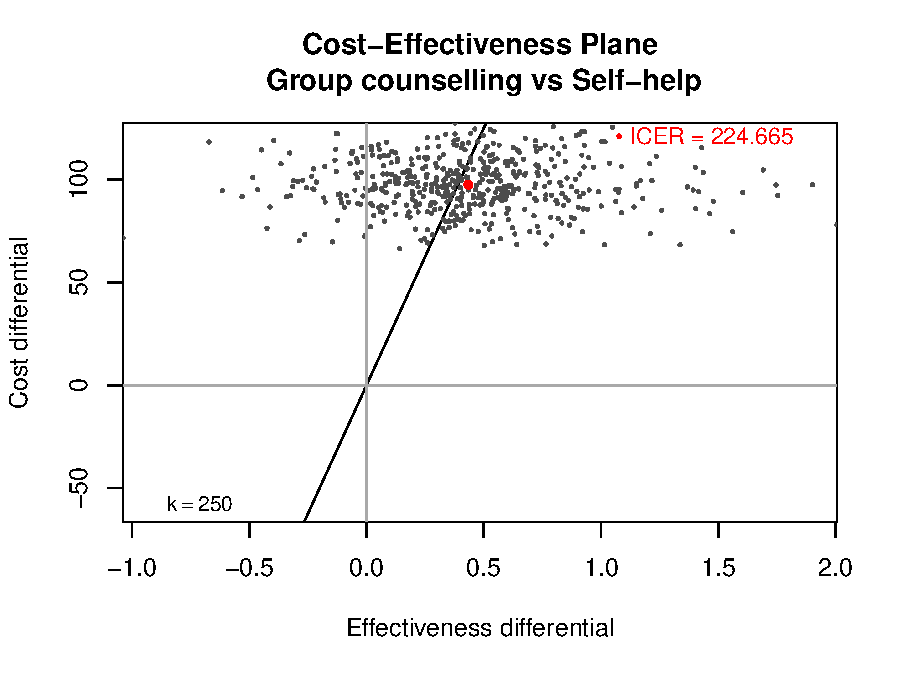
\includegraphics{C:/Users/n8tha/Documents/R/BCEA/vignettes/R_journal_examples_files/figure-latex/unnamed-chunk-5-1.pdf}

\begin{Shaded}
\begin{Highlighting}[]

\FunctionTok{setComparisons}\NormalTok{(bcea\_smoke) }\OtherTok{\textless{}{-}} \FunctionTok{c}\NormalTok{(}\DecValTok{1}\NormalTok{,}\DecValTok{3}\NormalTok{)}

\FunctionTok{ceplane.plot}\NormalTok{(bcea\_smoke, }\AttributeTok{wtp =} \DecValTok{250}\NormalTok{, }\AttributeTok{graph =} \StringTok{"ggplot2"}\NormalTok{)}
\end{Highlighting}
\end{Shaded}

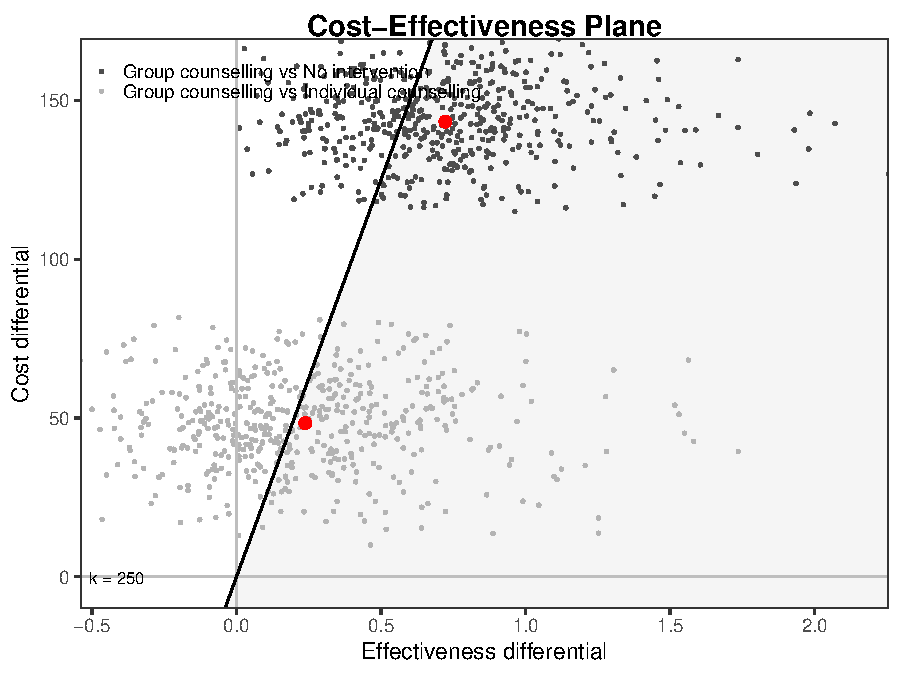
\includegraphics{C:/Users/n8tha/Documents/R/BCEA/vignettes/R_journal_examples_files/figure-latex/unnamed-chunk-5-2.pdf}

other plots

\begin{Shaded}
\begin{Highlighting}[]
\FunctionTok{eib.plot}\NormalTok{(bcea\_smoke)}
\end{Highlighting}
\end{Shaded}

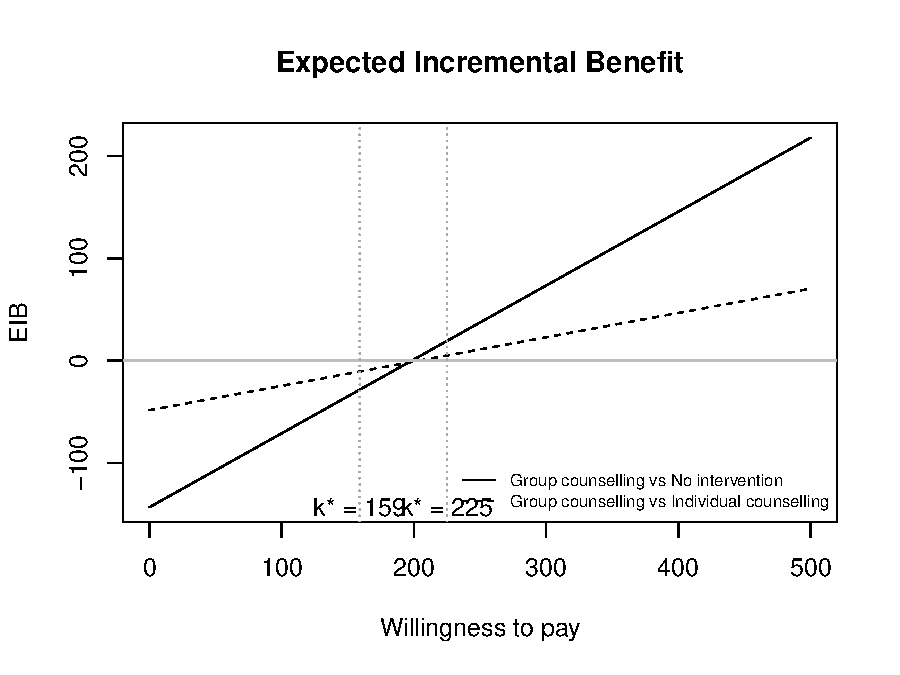
\includegraphics{C:/Users/n8tha/Documents/R/BCEA/vignettes/R_journal_examples_files/figure-latex/unnamed-chunk-6-1.pdf}

\begin{Shaded}
\begin{Highlighting}[]

\FunctionTok{contour}\NormalTok{(bcea\_smoke)}
\end{Highlighting}
\end{Shaded}

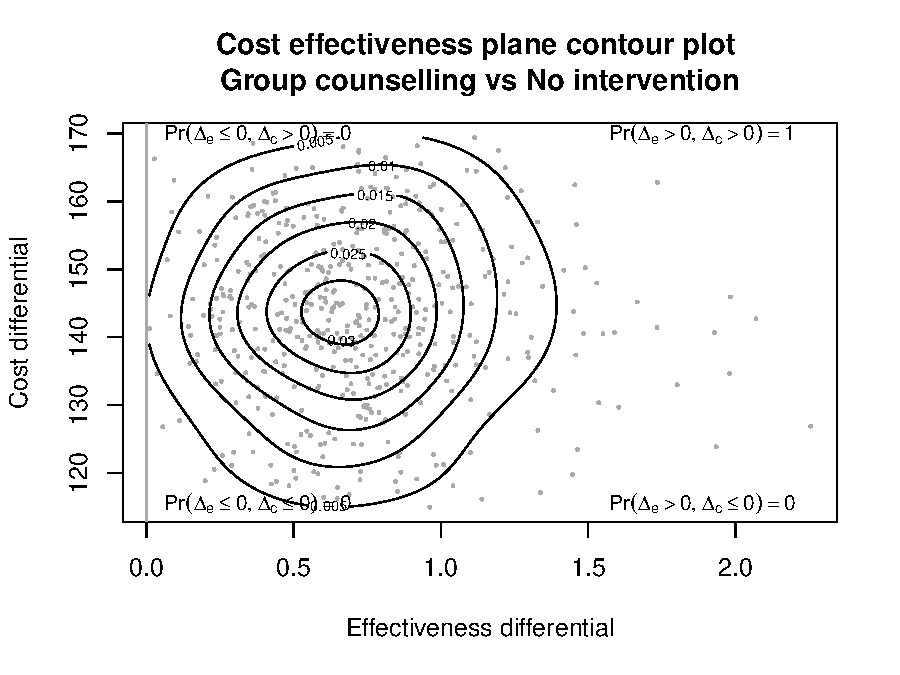
\includegraphics{C:/Users/n8tha/Documents/R/BCEA/vignettes/R_journal_examples_files/figure-latex/unnamed-chunk-6-2.pdf}

\begin{Shaded}
\begin{Highlighting}[]

\FunctionTok{ceac.plot}\NormalTok{(bcea\_smoke)}
\end{Highlighting}
\end{Shaded}

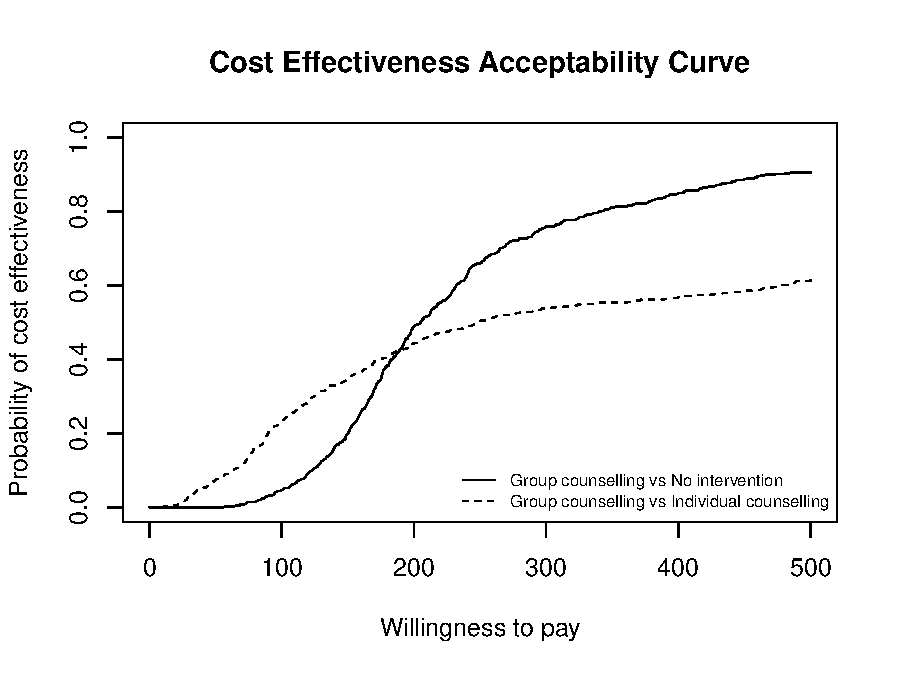
\includegraphics{C:/Users/n8tha/Documents/R/BCEA/vignettes/R_journal_examples_files/figure-latex/unnamed-chunk-6-3.pdf}

\begin{Shaded}
\begin{Highlighting}[]

\FunctionTok{ib.plot}\NormalTok{(bcea\_smoke)}
\CommentTok{\#\textgreater{} NB: k (wtp) is defined in the interval [0 {-} 500]}
\end{Highlighting}
\end{Shaded}

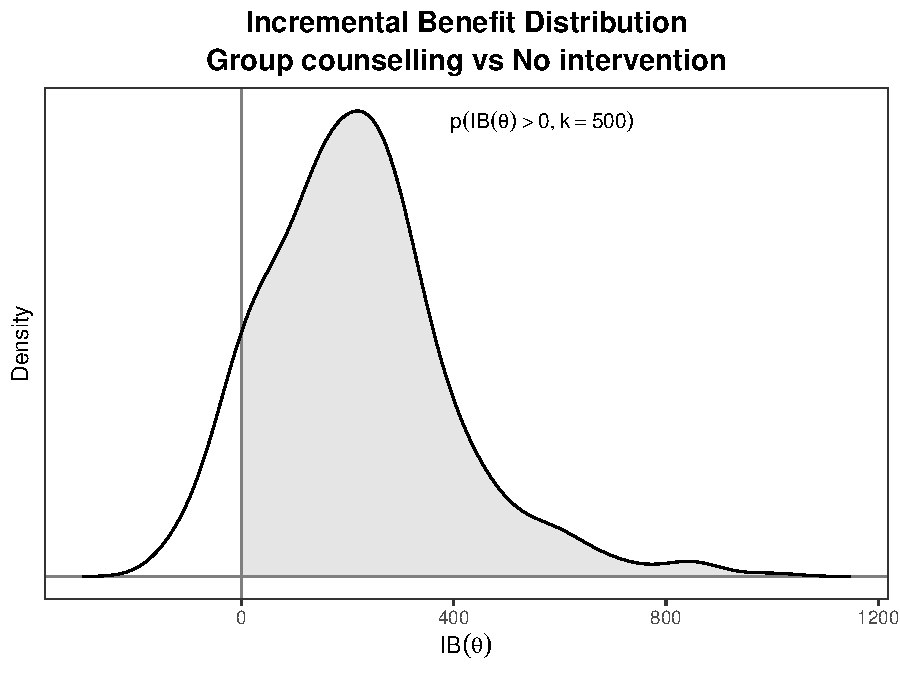
\includegraphics{C:/Users/n8tha/Documents/R/BCEA/vignettes/R_journal_examples_files/figure-latex/unnamed-chunk-6-4.pdf}

\begin{Shaded}
\begin{Highlighting}[]

\FunctionTok{ceef.plot}\NormalTok{(bcea\_smoke)}
\CommentTok{\#\textgreater{} }
\CommentTok{\#\textgreater{} Cost{-}effectiveness efficiency frontier summary }
\CommentTok{\#\textgreater{} }
\CommentTok{\#\textgreater{} Interventions on the efficiency frontier:}
\CommentTok{\#\textgreater{}                        Effectiveness   Costs Increase slope Increase angle}
\CommentTok{\#\textgreater{} Self{-}help                    0.48486  94.919         195.77         1.5657}
\CommentTok{\#\textgreater{} Individual counselling       0.72252 143.301         203.57         1.5659}
\CommentTok{\#\textgreater{} }
\CommentTok{\#\textgreater{} Interventions not on the efficiency frontier:}
\CommentTok{\#\textgreater{}                 Effectiveness Costs     Dominance type}
\CommentTok{\#\textgreater{} No intervention             0     0 Extended dominance}
\end{Highlighting}
\end{Shaded}

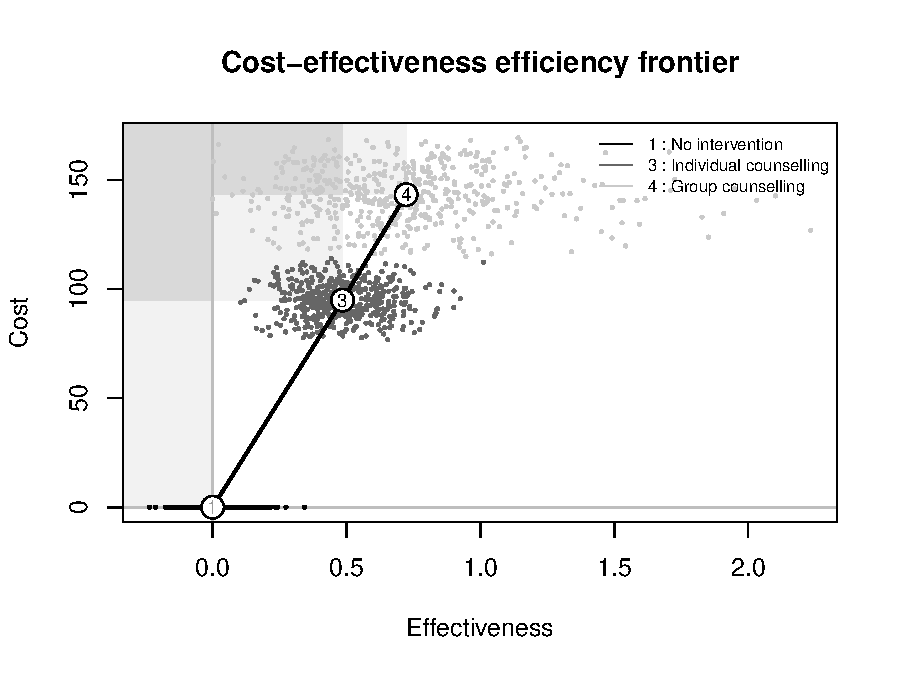
\includegraphics{C:/Users/n8tha/Documents/R/BCEA/vignettes/R_journal_examples_files/figure-latex/unnamed-chunk-6-5.pdf}

multiple simultaneous comparisons

\begin{Shaded}
\begin{Highlighting}[]
\NormalTok{bcea\_smoke }\OtherTok{\textless{}{-}} \FunctionTok{multi.ce}\NormalTok{(bcea\_smoke)}

\FunctionTok{ceac.plot}\NormalTok{(bcea\_smoke, }\AttributeTok{pos =} \StringTok{"topright"}\NormalTok{)}
\end{Highlighting}
\end{Shaded}

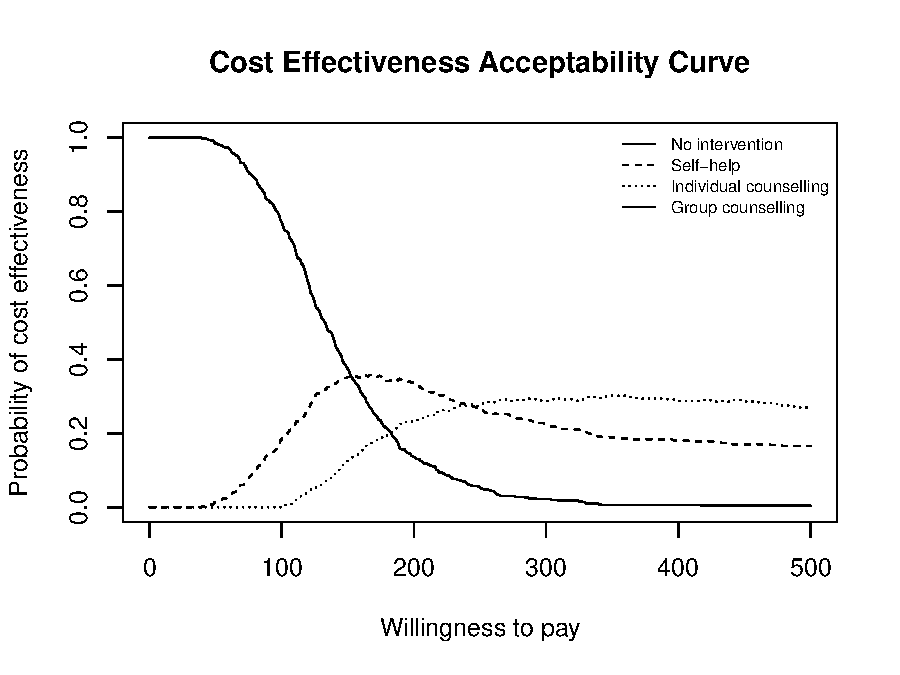
\includegraphics{C:/Users/n8tha/Documents/R/BCEA/vignettes/R_journal_examples_files/figure-latex/unnamed-chunk-7-1.pdf}

\begin{Shaded}
\begin{Highlighting}[]
\FunctionTok{ceaf.plot}\NormalTok{(bcea\_smoke)}
\end{Highlighting}
\end{Shaded}

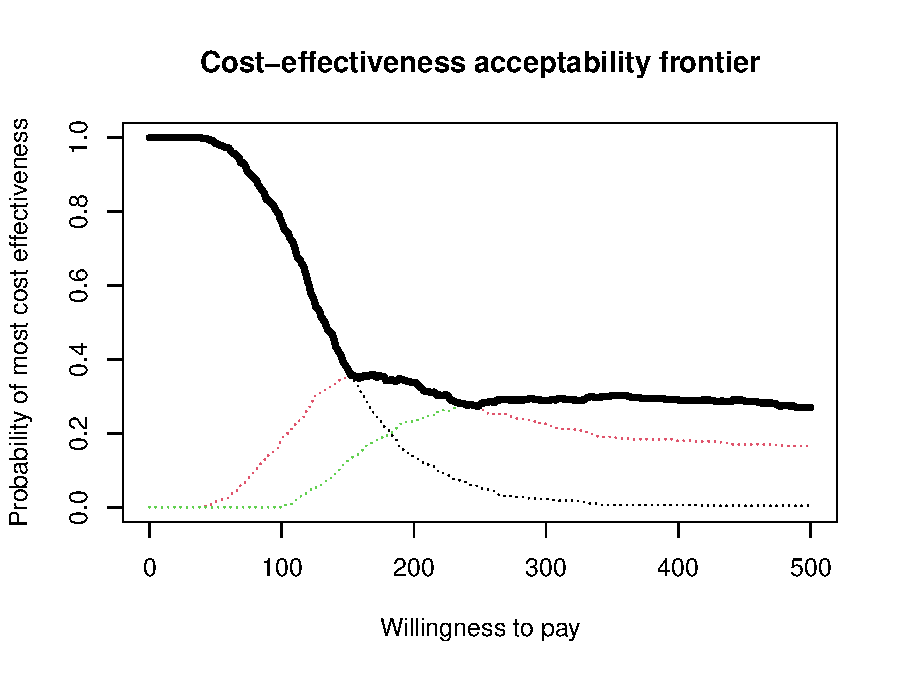
\includegraphics{C:/Users/n8tha/Documents/R/BCEA/vignettes/R_journal_examples_files/figure-latex/unnamed-chunk-7-2.pdf}

mixed strategy

\begin{Shaded}
\begin{Highlighting}[]
\FunctionTok{mixedAn}\NormalTok{(bcea\_smoke) }\OtherTok{\textless{}{-}} \FunctionTok{c}\NormalTok{(}\FloatTok{0.4}\NormalTok{, }\FloatTok{0.3}\NormalTok{, }\FloatTok{0.2}\NormalTok{, }\FloatTok{0.1}\NormalTok{)}
\FunctionTok{summary}\NormalTok{(bcea\_smoke, }\AttributeTok{wtp =} \DecValTok{250}\NormalTok{)}
\CommentTok{\#\textgreater{} }
\CommentTok{\#\textgreater{} Analysis of mixed strategy for willingness to pay parameter k = 250}
\CommentTok{\#\textgreater{} }
\CommentTok{\#\textgreater{} Reference intervention: Group counselling (10.00\% market share)}
\CommentTok{\#\textgreater{} Comparator intervention(s): No intervention (40.00\% market share)}
\CommentTok{\#\textgreater{}                           : Individual counselling (20.00\% market share)}
\CommentTok{\#\textgreater{} }
\CommentTok{\#\textgreater{} Loss in the expected value of information = 34.43}
\FunctionTok{evi.plot}\NormalTok{(bcea\_smoke, }\AttributeTok{graph =} \StringTok{"ggplot"}\NormalTok{, }\AttributeTok{pos =} \StringTok{"b"}\NormalTok{)}
\end{Highlighting}
\end{Shaded}

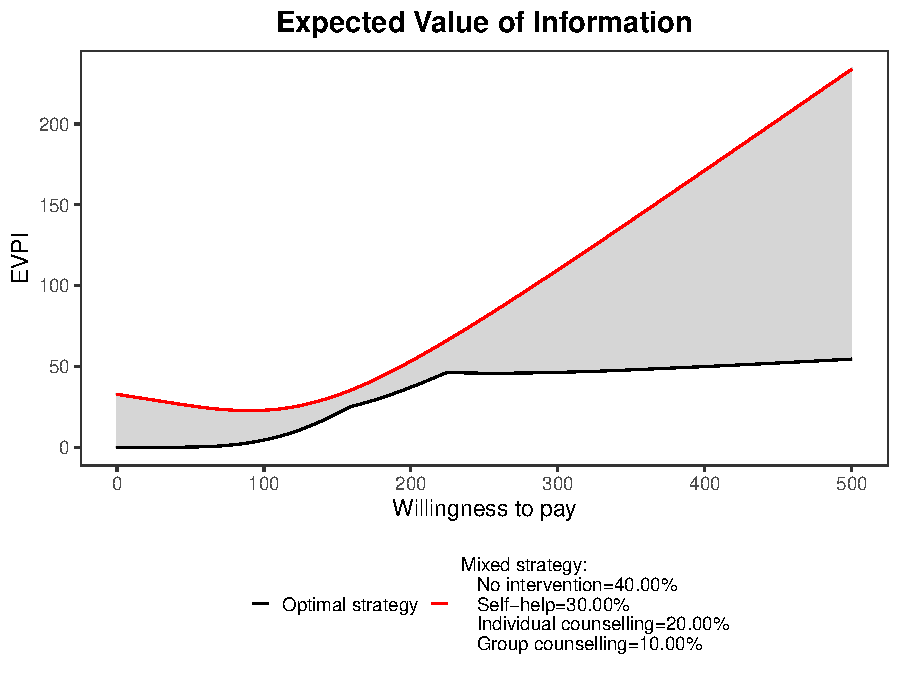
\includegraphics{C:/Users/n8tha/Documents/R/BCEA/vignettes/R_journal_examples_files/figure-latex/unnamed-chunk-8-1.pdf}

risk aversion

\begin{Shaded}
\begin{Highlighting}[]
\NormalTok{r }\OtherTok{\textless{}{-}} \FunctionTok{c}\NormalTok{(}\DecValTok{0}\NormalTok{, }\FloatTok{0.005}\NormalTok{, }\FloatTok{0.020}\NormalTok{, }\FloatTok{0.035}\NormalTok{)}
\FunctionTok{CEriskav}\NormalTok{(bcea\_smoke) }\OtherTok{\textless{}{-}}\NormalTok{ r}

\FunctionTok{plot}\NormalTok{(bcea\_smoke)}
\end{Highlighting}
\end{Shaded}

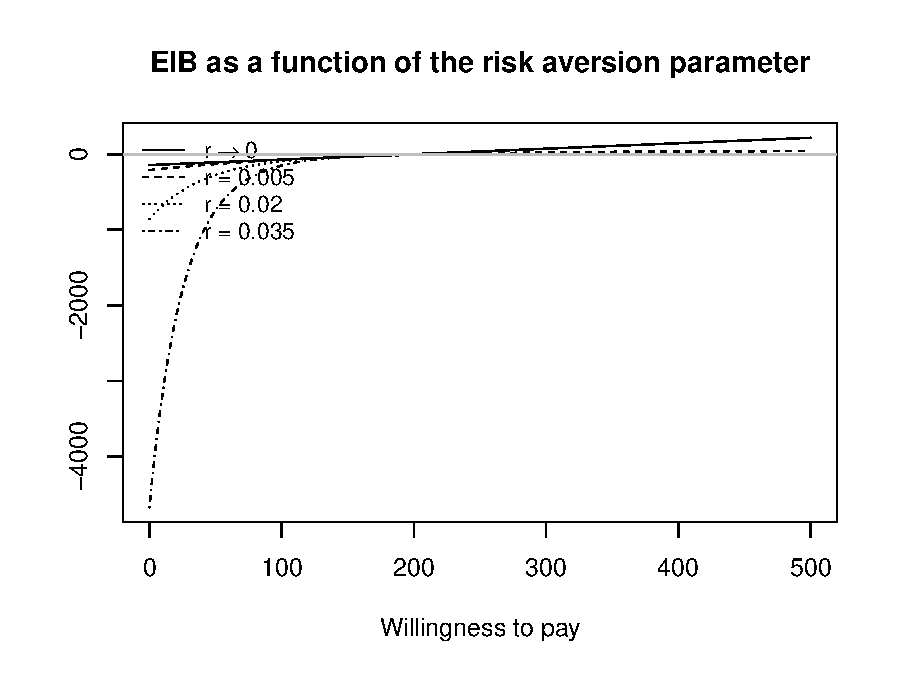
\includegraphics{C:/Users/n8tha/Documents/R/BCEA/vignettes/R_journal_examples_files/figure-latex/unnamed-chunk-9-1.pdf}
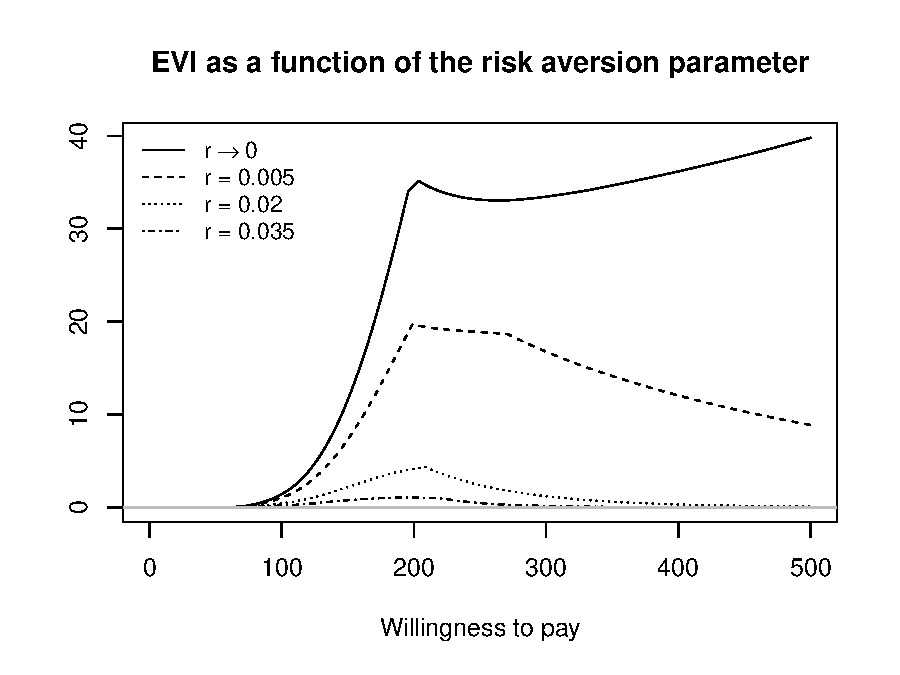
\includegraphics{C:/Users/n8tha/Documents/R/BCEA/vignettes/R_journal_examples_files/figure-latex/unnamed-chunk-9-2.pdf}

\hypertarget{influenza-vaccine-data}{%
\subsection{Influenza vaccine data}\label{influenza-vaccine-data}}

\begin{Shaded}
\begin{Highlighting}[]
\FunctionTok{data}\NormalTok{(Vaccine)}

\NormalTok{treats }\OtherTok{\textless{}{-}} \FunctionTok{c}\NormalTok{(}\StringTok{"Status quo"}\NormalTok{, }\StringTok{"Vaccination"}\NormalTok{)}
\NormalTok{bcea\_vacc }\OtherTok{\textless{}{-}} \FunctionTok{bcea}\NormalTok{(e, c, }\AttributeTok{ref =} \DecValTok{2}\NormalTok{, }\AttributeTok{interventions =}\NormalTok{ treats)}
\end{Highlighting}
\end{Shaded}

grid of plots

\begin{Shaded}
\begin{Highlighting}[]
\FunctionTok{plot}\NormalTok{(bcea\_vacc)}
\end{Highlighting}
\end{Shaded}

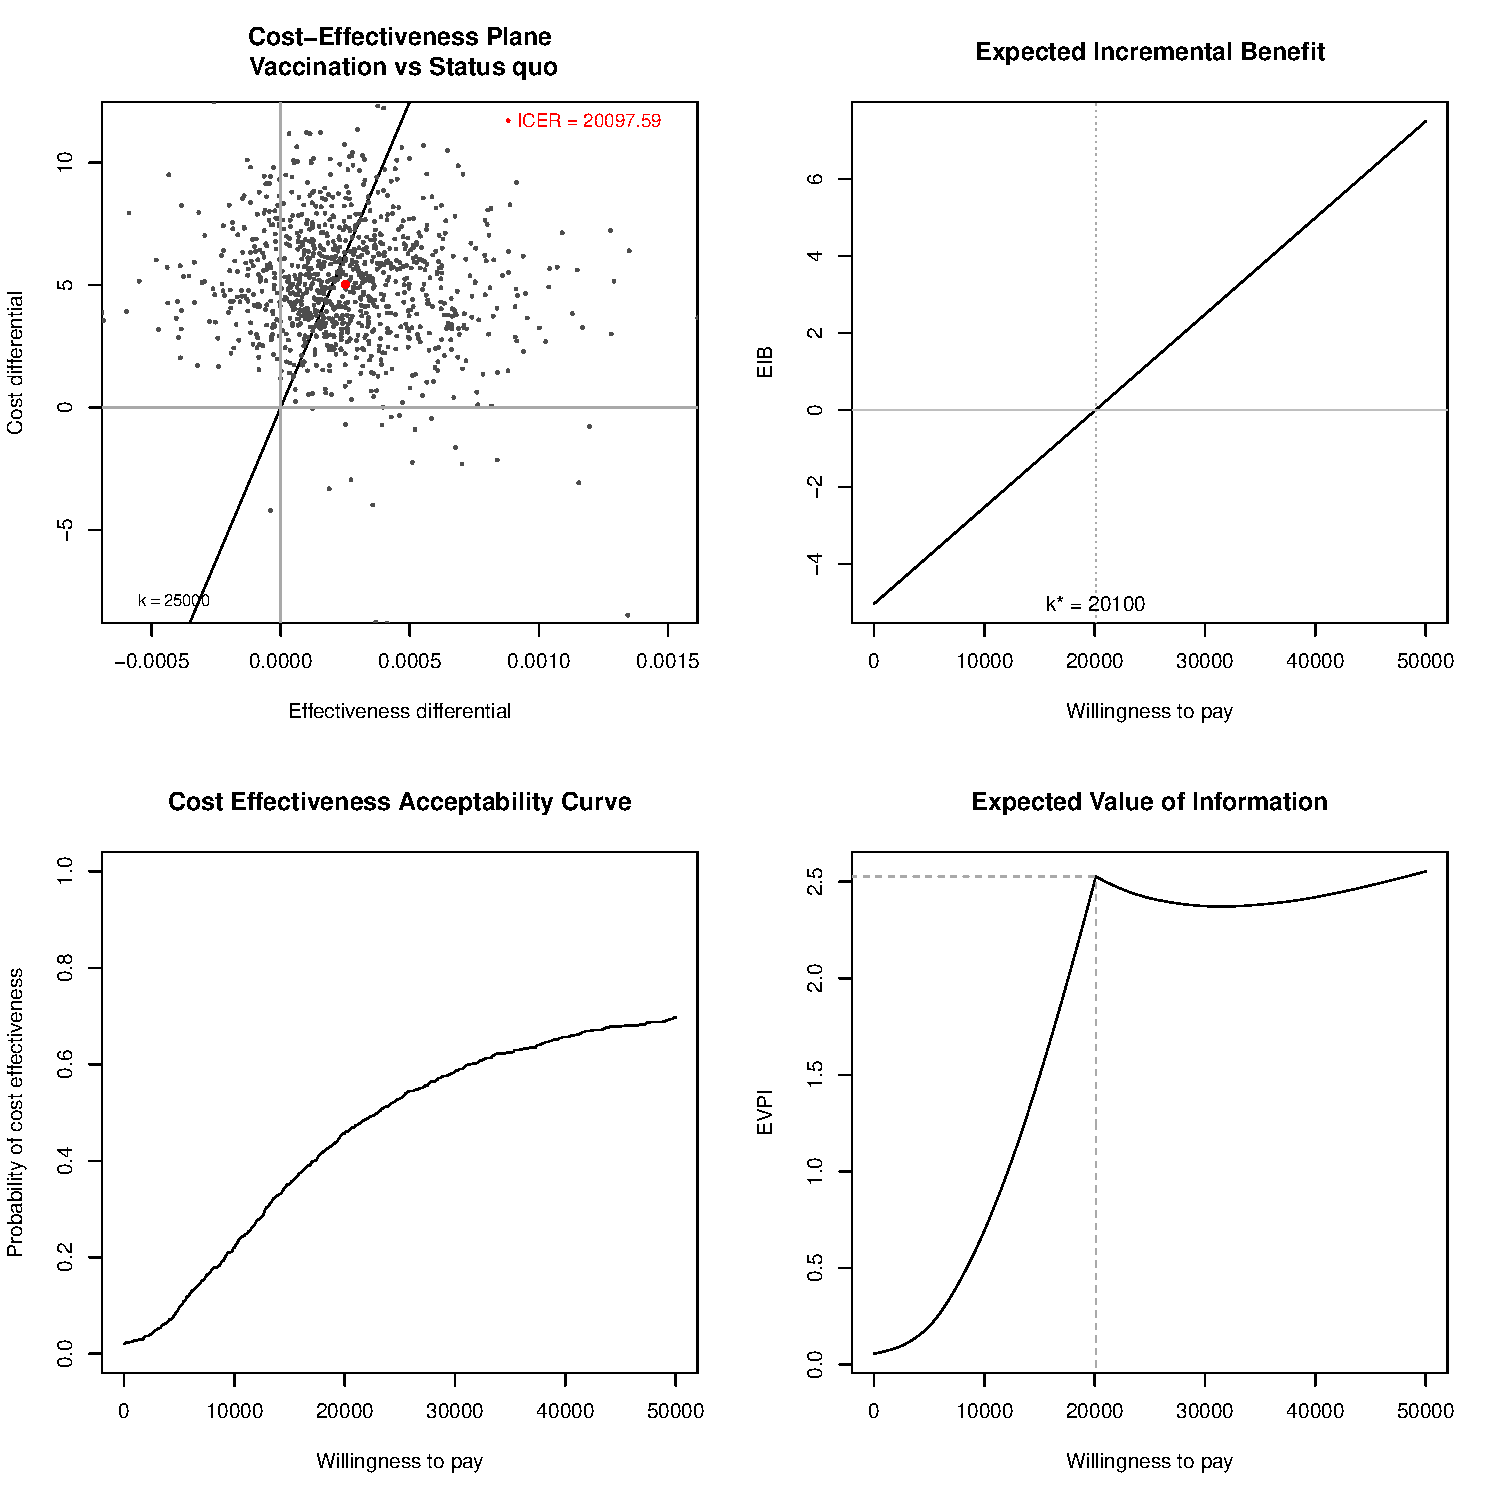
\includegraphics{C:/Users/n8tha/Documents/R/BCEA/vignettes/R_journal_examples_files/figure-latex/unnamed-chunk-11-1.pdf}

summary output

\begin{Shaded}
\begin{Highlighting}[]
\FunctionTok{summary}\NormalTok{(bcea\_vacc, }\AttributeTok{wtp =} \DecValTok{10000}\NormalTok{)}
\CommentTok{\#\textgreater{} }
\CommentTok{\#\textgreater{} Cost{-}effectiveness analysis summary }
\CommentTok{\#\textgreater{} }
\CommentTok{\#\textgreater{} Reference intervention:  Vaccination}
\CommentTok{\#\textgreater{} Comparator intervention: Status quo}
\CommentTok{\#\textgreater{} }
\CommentTok{\#\textgreater{} Optimal decision: choose Status quo for k \textless{} 20100 and Vaccination for k \textgreater{}= 20100}
\CommentTok{\#\textgreater{} }
\CommentTok{\#\textgreater{} }
\CommentTok{\#\textgreater{} Analysis for willingness to pay parameter k = 10000}
\CommentTok{\#\textgreater{} }
\CommentTok{\#\textgreater{}             Expected utility}
\CommentTok{\#\textgreater{} Status quo           {-}36.054}
\CommentTok{\#\textgreater{} Vaccination          {-}34.826}
\CommentTok{\#\textgreater{} }
\CommentTok{\#\textgreater{}                              EIB  CEAC  ICER}
\CommentTok{\#\textgreater{} Vaccination vs Status quo 1.2284 0.529 20098}
\CommentTok{\#\textgreater{} }
\CommentTok{\#\textgreater{} Optimal intervention (max expected utility) for k = 10000: Status quo}
\CommentTok{\#\textgreater{}            }
\CommentTok{\#\textgreater{} EVPI 3.0287}
\FunctionTok{head}\NormalTok{(}\FunctionTok{sim\_table}\NormalTok{(bcea\_vacc, }\AttributeTok{wtp =} \DecValTok{25000}\NormalTok{)}\SpecialCharTok{$}\NormalTok{Table)}
\CommentTok{\#\textgreater{}          U1        U2        U*      IB2\_1       OL         VI}
\CommentTok{\#\textgreater{} 1 {-}36.57582 {-}38.71760 {-}36.57582 {-}2.1417866 2.141787  {-}1.135907}
\CommentTok{\#\textgreater{} 2 {-}27.92514 {-}27.67448 {-}27.67448  0.2506573 0.000000   7.765431}
\CommentTok{\#\textgreater{} 3 {-}28.03024 {-}33.37394 {-}28.03024 {-}5.3436963 5.343696   7.409665}
\CommentTok{\#\textgreater{} 4 {-}53.28408 {-}47.13734 {-}47.13734  6.1467384 0.000000 {-}11.697432}
\CommentTok{\#\textgreater{} 5 {-}43.58389 {-}40.40469 {-}40.40469  3.1791976 0.000000  {-}4.964782}
\CommentTok{\#\textgreater{} 6 {-}42.37456 {-}33.08547 {-}33.08547  9.2890987 0.000000   2.354444}
\end{Highlighting}
\end{Shaded}

value of information

\begin{Shaded}
\begin{Highlighting}[]
\FunctionTok{evi.plot}\NormalTok{(bcea\_vacc)}
\end{Highlighting}
\end{Shaded}

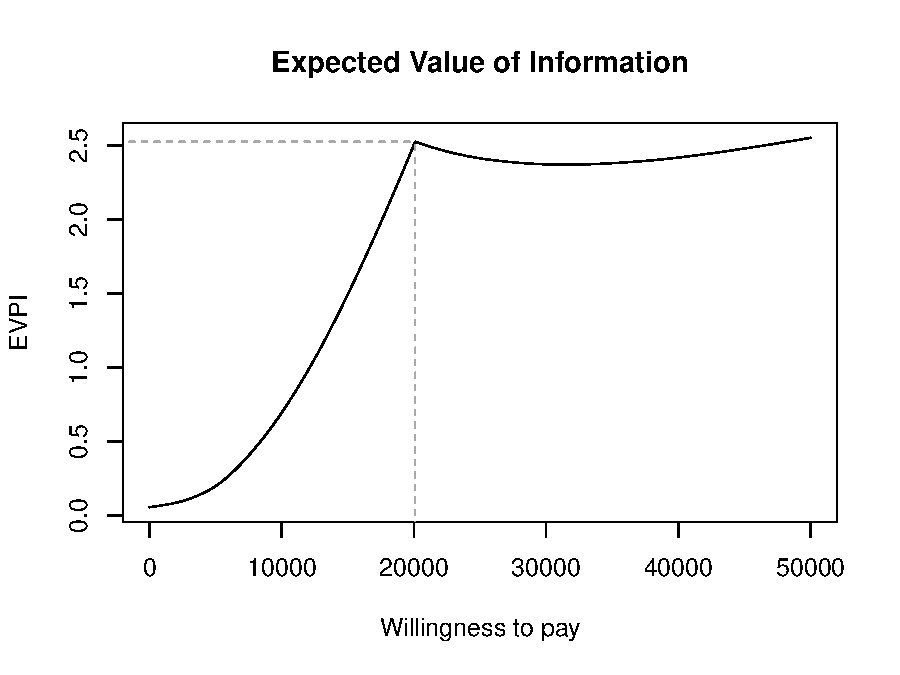
\includegraphics{C:/Users/n8tha/Documents/R/BCEA/vignettes/R_journal_examples_files/figure-latex/unnamed-chunk-13-1.pdf}

\begin{Shaded}
\begin{Highlighting}[]
\NormalTok{inp }\OtherTok{\textless{}{-}} \FunctionTok{createInputs}\NormalTok{(vaccine, }\AttributeTok{print\_is\_linear\_comb =} \ConstantTok{FALSE}\NormalTok{)}
\FunctionTok{info.rank}\NormalTok{(bcea\_vacc, inp)}
\end{Highlighting}
\end{Shaded}

\begin{Shaded}
\begin{Highlighting}[]
\NormalTok{EVPPI }\OtherTok{\textless{}{-}} \FunctionTok{evppi}\NormalTok{(bcea\_vacc, }\FunctionTok{c}\NormalTok{(}\StringTok{"beta.1."}\NormalTok{, }\StringTok{"beta.2."}\NormalTok{), inp}\SpecialCharTok{$}\NormalTok{mat)}
\FunctionTok{plot}\NormalTok{(EVPPI)}
\end{Highlighting}
\end{Shaded}


\end{document}
